\subsection{Vergelijking van een rechte}


Het vlak is voorzien van een Euclidisch assenstelsel met oorsprong $O$.
In het vlak is $l$ een rechte door $O$ verschillend van \'e\'en van de assen van het assenstelsel.
Je neemt op $l$ twee verschillende punten $Q(x_1;y_1)$ en $R(x_2;y_2)$ allebei verschillend van $O$.
Je noemt $Q_1$ (resp.$R_1$) de loodrechte projectie van $Q$ (resp. $R$) op de $x$-as.
Omdat de rechthoekige driehoeken $OQQ_1$ en $ORR_1$ even grote overeenkomstige hoeken hebben zijn ze gelijkvormig.

\gewonefiguur{height=5cm}{4_opp_inhoud_an_meetk/inputs/AMTekst4Fig1}

%\begin{figure}[!htb]
%\begin{center}
%\includegraphics[height=5 cm]{4_opp_inhoud_an_meetk/inputs/AMTekst4Fig1}
%\end{center}
%\end{figure} 
Hieruit volgt dat de verhoudingen van lengten van overeenkomstige zijden gelijk zijn, dus
\[
\frac {\vert RR_1 \vert}{\vert QQ_1 \vert}=\frac {\vert OR_1 \vert}{\vert OQ_1 \vert} \text { .}
\]
In termen van co\"ordinaten bekom je
\[
\frac {\vert y_1 \vert}{\vert y_2 \vert}=\frac {\vert x_1 \vert}{\vert x_2 \vert} \text { en dus } \frac {\vert y_1 \vert}{\vert x_1 \vert}=\frac {\vert y_2 \vert}{\vert x_2 \vert} \text { .}
\]
Merk op dat op de linkse figuur voor een punt $P(x;y)$ op $l$ verschillende van $O$ steeds geldt dat $\frac {y}{x}>0$ terwijl op de rechtse figuur steeds geldt $\frac {y}{x}<0$.
De tekens van $\frac {y_1}{x_1}$ en $\frac {y_2}{x_2}$ zijn dus steeds gelijk en je bekomt daardoor zelfs
\[
\frac {y_1}{x_1} = \frac{y_2}{x_2} \text { .}
\]
Je bekomt hieruit dat een getal $m \in \mathbb{R}_0$ bestaat zodat voor ieder punt $P(x;y)$ op $l$ verschillende van $O$ geldt
\[
\frac {y}{x}=m \text { en dus } y=mx \text { .}
\]
Deze laatste vergelijking is een nodige en voldoende voorwaarde opdat een punt $P(x;y)$ in het vlak tot de rechte $l$ behoort.
Het is een vergelijking van $l$.
Voor $l$ als op de linkse figuur is $m>0$ en voor $l$ als op de rechtse figuur is $m<0$.

Als $l$ de $x$-as is dan behoort een punt $P(x;y)$ van het vlak tot $l$ als en alleen als $y=0$.
Dit laatste is dan een vergelijking van $l$ (dus van de $x$-as).
Merk op, door $m=0$ te nemen in vorig resultaat bekom je dat je de vergelijking eveneens in de vorm $y=0.x$ kan schrijven.

Als $l$ de $y$-as is dan behoort een punt $P(x;y)$ van het vlak tot $l$ als en alleen als $x=0$.
Dit laatste is dan een vergelijking van $l$ (dus van de $y$-as).
Merk op, er is geen enkel getal $m$ zodat je die laatste vergelijking kunt schrijven in de vorm $y=mx$.

Voor een rechte $l$ door de oorsprong is $\alpha$ een geori\"enteerde hoek van de $x$-as naar $l$.
\begin{itemize}
\item Een geori\"enteerde hoek is positief in tegenwijzerszin en negatief in wijzerszin.
\item De hoek $\alpha$ is slechts op een veelvoud van $180^o$ ($\pi$ radialen) na bepaald (zie de figuur).
\end{itemize}
\gewonefiguur{height=5cm}{4_opp_inhoud_an_meetk/inputs/AMTekst4Fig2}

Zulke geori\"enteerde hoek komt overeen met een punt op de goniometrische cirkel.
Uit de constructie van de tangens bekom je dat $(1; \tan \alpha)$ de co\"ordinaten zijn van een punt op $l$ (als $l$ niet de $y$-as is).
Omdat de punten van $l$ moeten voldoen aan een vergelijking $y=mx$ bekom je $m=\tan \alpha$.

Samengevat bekomen we het volgende resultaat.
De vergelijking van een rechte $l$ door de oorsprong $O$ verschillend van de $y$-as is $y=(\tan \alpha )x$.
Hierbij is $\alpha$ de geori\"enteerde hoek tussen de positieve $x$-as en de rechte $l$.
De vergelijking van de $y$-as is $x=0$.\\

Een rechte $l$ die niet door de oorsprong $O$ gaat en niet evenwijdig is met de $y$-as snijdt de $y$-as in een punt $Q(0;q)$.
De rechte $l'$ door de oorsprong $O$ die evenwijdig is aan $l$ heeft een vergelijking $y=mx$.

Voor een punt $P(x;y)$ op $l$ is $P'$ de projectie van $P$ op $l$ evenwijdig met de $y$-as.

\gewonefiguur{height=5cm}{4_opp_inhoud_an_meetk/inputs/AMTekst4Fig3}

%\begin{figure}[!htb]
%\begin{center}
%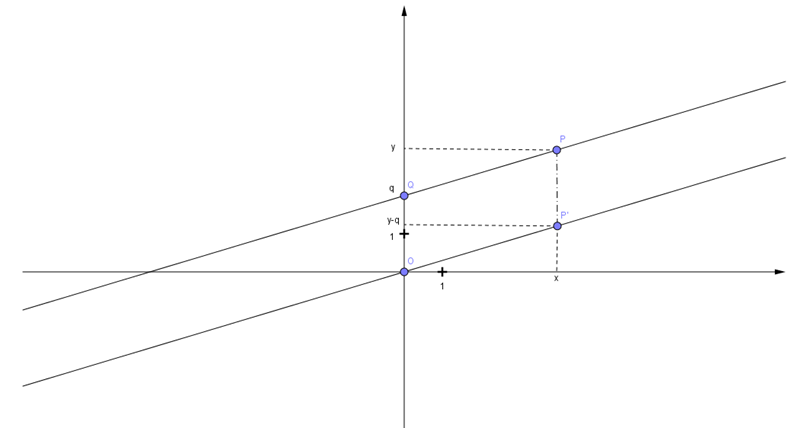
\includegraphics[height=8 cm]{4_opp_inhoud_an_meetk/inputs/AMtekst4Fig3}
%\end{center}
%\end{figure} 
De co\"ordinaten van $P'$ zijn $(x;y-q)$ en omdat $P'$ tot de rechte $l'$ met vergelijking $y=mx$ behoort moet $y-q=mx$.
Je bekomt dat een nodige en voldoende voorwaarde opdat een $P(x;y)$ in het vlak tot de rechte $l$ behoort is $y=mx+q$.
Dat getal $m$ is $\tan \alpha$ met $\alpha$ de geori\"enteerde hoek tussen de positieve $x$-as en de rechte $l$.
Je noemt $m$ de richtinsco\"effici\"ent van $l$ en je noteert $m=\rico (l)$.

Je besluit : een vergelijking van $l$ is $y=mx+q$.

Indien $l$ een rechte is evenwijdig met de $y$-as dan bestaat $a \in \mathbb{R}$ zodat $l$ bestaat uit alle punten $P(x;y)$ in het vlak waarvoor $x=a$.
In dat geval in $x=a$ een vergelijking van $l$.
Merk op dat je zulke vergelijking niet kunt schrijven in vorm $y=mx+q$, zulke rechte $l$ heeft geen richtingsco\"effici\"ent.

\begin{opmerking}
	Als $\rico(l)=m$ en $P_0(x_0;y_0)$ is een punt op $l$ dan is
\[
y-y_0=m(x-x_0)
\]
een vergelijing van $l$.
Duidelijk voldoen de co\"ordinaten van $P_0$ aan de vergelijking.
Je kunt de vergelijking herleiden tot de vorm $y=mx+(y_0-mx_0)$.
Dit is van de vorm $y=mx+q$ met $q=y_0-mx_0$ en dus de vergelijking van een rechte.
In die laatste vorm herken je ook dat $m$ de richtinsco\"effici\"ent is van die rechte.\\
\end{opmerking}

%Aan de makers van de cursus: ik stel voor hier een filmpje toe te voegen.Dit filmpje moet de invloed van $l$ en $m$ op de ligging van de rechte met vergelijking $y=mx+q$ illustreren.
%Wat nu volgt is een voorstel voor het scenario van dat filmpje.
%
% \underline{Fimpje}
%
%$y=mx$ tekenen waarbij $m$ van -3 naar 3 toeneemt (toename van $m$ met vaste snelheid; als mogelijk op voorhand vermelden wat gaat gebeuren (met geluid dus) en daarbij vermelden dat de richting zelf het snelste verandert als de rico dicht bij 0 is).
%
%$y=2x+q$ tekenen waarbij $q$ van -3 naar 3 toeneemt. Ook snijpunt met de $y$-as duidelijk erbij tekenen (toename van $q$ opnieuw met constante snelheid, op voorhand vertellen wat gaat gebeuren en opmerken dat ook het snijpunt met de $y$-as met constante snelheid zal bewegen).
%
%$y-1=-\frac {1}{2} (x-a)$ tekenen waarbij $a$ van -3 naar 3 toeneemt. Ook het punt met $y$-co\"ordinaat 1 erbij tekenen (toename van $a$ opnieuw met constante snelheid, op voorhand vertellen wat gaat gebeuren en opmerken dat ook het punt met $y$-co\"ordinaat gelijk aan 1 met constante snelheid zal bewegen).
%
%Hiermee be\"eindigt dan het filmpje.\\

%Aan de makers van de cursus : mijn voorstel is om het volgende voorbeeld met topcamera te maken.

\subsection{Vergelijking rechte - voorbeeld}
Zie filmpje MOOC.

\subsection{Vergelijking rechte met richting en door gegeven punt - extra voorbeelden}
Zie filmpje MOOC.

\subsection{Vergelijking rechte met richting en door gegeven punt - extra voorbeelden}

\begin{voorbeeld}
Geef een vergelijking van de rechte $l$ zodat de geori\"enteerde hoek tussen de positieve $x$-as en $l$ gelijk is aan $30^o$ en zodat het punt $P(2;-5)$ tot  $l$ behoort.
Geef eveneens de co\"ordinaten van het snijpunt van $l$ met de $x$-as en met de $y$-as.

\gewonefiguur{height=5cm}{4_opp_inhoud_an_meetk/inputs/AMTekst4Fig4}

%\begin{figure}[!htb]
%\begin{center}
%\includegraphics[height=5 cm]{4_opp_inhoud_an_meetk/inputs/AMTekst4Fig4}
%\caption{Voorbeeld 1.}
%\label{fig4.2.9_fig4}
%\end{center}
%\end{figure} 

Er geldt $\rico (l)=\tan (30^o)=\frac {1}{\sqrt{3}}$.
De vergelijking van $l$ is $y-(-5)=\frac{1}{\sqrt{3}}(x-2)$ en je bekomt
\[
y=\frac{1}{\sqrt{3}}x-5-\frac{2}{5} \text { dus } y=0,577x-6,155 \text { .}
\]
Omdat $q=-6,155$ is heeft het snijpunt $A$ met de $y$-as co\"ordinaten $(0;-6,155)$.
(Dit vind je ook door $x=0$ in de vergelijking in te vullen.)
Op de $x$-as is $y=0$. Voor het snijpunt $B$ met de $x$-as geldt daarom $0,577x-6,155=0$.
Je bekomt
\[
x=\frac{6,155}{0,577}=10,667 \text { .}
\]
Het snijpunt $B$ met de $x$-as heeft co\"ordinaten $(10,667;0)$.\\

We stellen nu de vergelijking op van een rechte door twee gegeven verschillende punten $P_1(x_1;y_1)$ en $P_2(x_2;y_2)$.
Als $x_1=x_2$ dan is de rechte evenwijdig met de $y$-as en de vergelijking is $x=a$ (met $a=x_1$).

Stel dat $x_1 \neq x_2$ (de rechte is dus niet evenwijdig met de $y$-as).
De rechte heeft een vergelijking van de vorm $y=mx+q$.
Deze vergelijking moet gelden als je de co\"ordinaten van $P_1$ en $P_2$ invult.
Dit geeft volgende gelijkheden:
\[
y_1=m.x_1+q \text { en } y_2=m.x_2+q \text { .}
\]
Neem je van beide leden van deze twee gelijkheden telkens het verschil dan bekom je
\[
y_2-y_1=m.(x_2-x_1) 
\]
en omdat $x_1 \neq x_2$ bekom je
\[
\rico (P_1P_2)=m=\frac {y_2-y_1}{x_2-x_1} \text { .}
\]
Je bekomt als vergelijking van de rechte $P_1P_2$
\[
y-y_1=\frac {y_2-y_1}{x_2-x_1} (x-x_1) \text { .}
\]\\

\end{voorbeeld}


\begin{voorbeeld}
Geef een vergelijking van de rechte $l$ door de punten $P(3;5)$ en $Q(-2;4)$.

\gewonefiguur{height=5cm}{4_opp_inhoud_an_meetk/inputs/AMTekst4Fig5}

%\begin{figure}[!htb]
%\begin{center}
%\includegraphics[height=5 cm]{4_opp_inhoud_an_meetk/inputs/AMTekst4Fig5}
%\caption{Voorbeeld 1.}
%\label{fig4.2.9_fig5}
%\end{center}
%\end{figure}

Invullen in voorgaande formule geeft
\[
y-5=\frac{4-5}{-2-3}(x-3)
\]
en mits wat rekenwerk bekom je hieruit
\[
y=\frac{1}{5}x+\frac{22}{5} \text { .}
\]\\

Je kunt een vergelijking van een rechte steeds schrijven in de vorm $ax+by+c=0$ met $a$ en $b$ niet allebei 0.
Omgekeerd, een vergelijking van de vorm $ax+by+c=0$ met $a$ en $b$ niet allebei gelijk aan 0 steeds een vergelijking van een rechte.
\begin{itemize}
\item Indien $b=0$ dan is $a \neq 0$ en je kunt de vergelijking omvormen tot $x=-\frac{c}{a}$.
Je bekomt een rechte evenwijdig met de $y$-as (door het punt $(-\frac{c}{a};0)$).
\item Indien $b \neq 0$ dan kun je de vergelijking omvormen tot
\[
y=\left( -\frac{a}{b}  \right)x+\left(  -\frac{c}{b} \right) \text { .}
\]
Je bekomt de rechte met richtingsco\"effici\"ent $-\frac {a}{b}$ door het punt $(0; -\frac{c}{b})$.
\end{itemize}

\end{voorbeeld}